% Attention matrix heatmap for "the cat sat on the mat"
% Shows self-attention scores as a 6×6 matrix
% Compile with:
%   pdflatex attention_matrix.tex
%   convert -density 200 attention_matrix.pdf -quality 95 attention_matrix.png

\documentclass[tikz,border=10pt]{standalone}
\usepackage{tikz}
\usetikzlibrary{matrix}

% Define color gradient for attention scores (white -> blue)
\definecolor{att0}  {RGB}{245,245,250}  % very low  (0.0-0.1)
\definecolor{att1}  {RGB}{220,230,245}  % low       (0.1-0.2)
\definecolor{att2}  {RGB}{180,200,230}  % medium    (0.2-0.3)
\definecolor{att3}  {RGB}{130,160,210}  % high      (0.3-0.5)
\definecolor{att4}  {RGB}{70,110,180}   % very high (0.5+)

\begin{document}
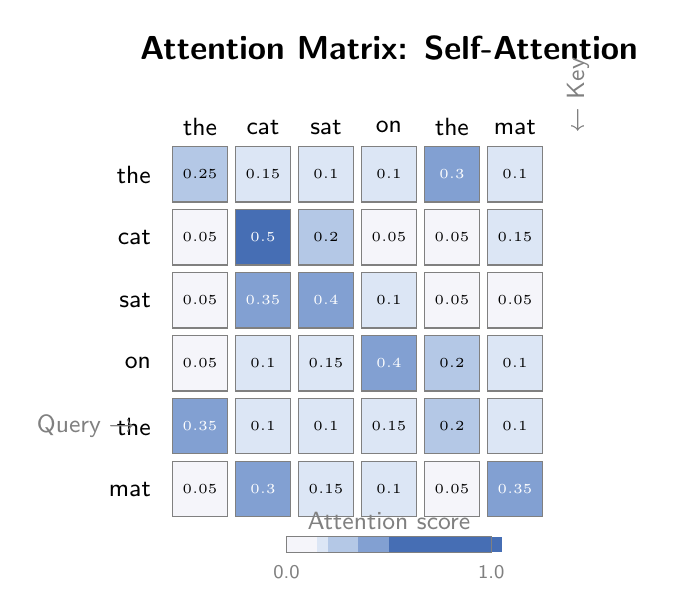
\begin{tikzpicture}[font=\sffamily]

% ── Title ────────────────────────────────────────────────────────
\node[font=\large\bfseries\sffamily] at (3.5, 4.8)
    {Attention Matrix: Self-Attention};

% Define cell size
\def\cellsize{0.8cm}

% Words
\def\words{{"the", "cat", "sat", "on", "the", "mat"}}

% Attention matrix (estimated scores)
% Each row shows how much that word attends to all words
% Rows must sum to 1.0 (softmax normalization)
\def\attmatrix{{
    {0.25, 0.15, 0.10, 0.10, 0.30, 0.10},  % the₁ → attends to "the₂" and itself
    {0.05, 0.50, 0.20, 0.05, 0.05, 0.15},  % cat → attends to itself, "sat", "mat"
    {0.05, 0.35, 0.40, 0.10, 0.05, 0.05},  % sat → attends to itself and "cat"
    {0.05, 0.10, 0.15, 0.40, 0.20, 0.10},  % on → attends to itself, "the₂", "mat"
    {0.35, 0.10, 0.10, 0.15, 0.20, 0.10},  % the₂ → attends to "the₁" and itself
    {0.05, 0.30, 0.15, 0.10, 0.05, 0.35}   % mat → attends to itself and "cat"
}}

% Function to get color based on score
\newcommand{\getcolor}[1]{%
    \pgfmathparse{#1 < 0.1 ? "att0" : (#1 < 0.2 ? "att1" : (#1 < 0.3 ? "att2" : (#1 < 0.5 ? "att3" : "att4")))}%
    \pgfmathresult%
}

% Draw column labels (top)
\foreach \j in {0,...,5} {
    \pgfmathsetmacro{\word}{\words[\j]}
    \node[font=\small\sffamily] at ({1.1 + \j * 0.8}, 3.8) {\word};
}

% Draw row labels (left)
\foreach \i in {0,...,5} {
    \pgfmathsetmacro{\word}{\words[\i]}
    \node[font=\small\sffamily, anchor=east] at (0.6, {3.2 - \i * 0.8}) {\word};
}

% Draw the matrix cells
\foreach \i in {0,...,5} {
    \foreach \j in {0,...,5} {
        \pgfmathsetmacro{\score}{\attmatrix[\i][\j]}
        \pgfmathsetmacro{\xpos}{1.1 + \j * 0.8}
        \pgfmathsetmacro{\ypos}{3.2 - \i * 0.8}

        % Determine color
        \pgfmathparse{\score < 0.1 ? "att0" : (\score < 0.2 ? "att1" : (\score < 0.3 ? "att2" : (\score < 0.5 ? "att3" : "att4")))}
        \edef\cellcolor{\pgfmathresult}

        % Draw cell
        \fill[\cellcolor] ({\xpos - 0.35}, {\ypos - 0.35}) rectangle ({\xpos + 0.35}, {\ypos + 0.35});
        \draw[gray, thin] ({\xpos - 0.35}, {\ypos - 0.35}) rectangle ({\xpos + 0.35}, {\ypos + 0.35});

        % Add score text
        \pgfmathparse{\score >= 0.3 ? "white" : "black"}
        \edef\textcolor{\pgfmathresult}
        \node[font=\tiny\sffamily, text=\textcolor] at (\xpos, \ypos) {\pgfmathprintnumber[fixed, precision=2]{\score}};
    }
}

% Axis labels
\node[font=\small\sffamily, anchor=east, text=gray] at (0.4, 0.0) {Query →};
\node[font=\small\sffamily, text=gray, rotate=90] at (5.9, 4.2) {← Key};

% Color bar legend
\node[font=\small\sffamily, text=gray] at (3.5, -1.2) {Attention score};

% Draw mini color gradient
\foreach \x in {0,...,20} {
    \pgfmathsetmacro{\val}{\x / 20}
    \pgfmathparse{\val < 0.1 ? "att0" : (\val < 0.2 ? "att1" : (\val < 0.3 ? "att2" : (\val < 0.5 ? "att3" : "att4")))}
    \edef\gradcolor{\pgfmathresult}
    \fill[\gradcolor] ({2.2 + \x * 0.13}, -1.6) rectangle ({2.2 + (\x + 1) * 0.13}, -1.4);
}
\draw[gray] (2.2, -1.6) rectangle (4.8, -1.4);
\node[font=\scriptsize\sffamily, text=gray, anchor=north] at (2.2, -1.65) {0.0};
\node[font=\scriptsize\sffamily, text=gray, anchor=north] at (4.8, -1.65) {1.0};

\end{tikzpicture}
\end{document}
